\documentclass{ctexart}  
\usepackage[left=2cm,right=1.97cm,top=2cm,bottom=2cm]{geometry}	
\usepackage{ctex}
\usepackage{palatino}
\usepackage{lipsum}
\usepackage{graphicx}
\usepackage{hyperref}
\usepackage{tabularray}
\usepackage{color}
\usepackage{listings}
\usepackage{float}
\usepackage{xcolor}

\title{\heiti \zihao{2}实验二:Shell 工具和脚本、编辑器(Vim)、
数据整理学习实验报告}
\author{\kaishu \zihao{-4} 邓林\qquad 23020007014\\
\songti \zihao{-5}中国海洋大学 \qquad 23软件工程 }
\date{}
\ctexset{section={format={\heiti \zihao{4}}},
subsection={format={ \songti \zihao{4}},beforeskip=0pt,afterskip=0pt},
subsubsection={format={\kaishu \zihao{4}},beforeskip=0pt ,afterskip=0pt}}
%%%%%%%%%%%%%%%%%%%%%%%%%

\begin{document}
    \maketitle
\vspace{-20pt}\begin{abstract}				
    本实验报告主要记录了作者通过课程网站及B站学习Shell 工具和脚本、编辑器(Vim)、
    数据整理的学习过程以及心得。
\end{abstract}

\section{实验内容}
主要学习了1.Shell语法和简单的使用;2.vim编辑器的使用方法以及光标移动快捷键等;3.数据整理及正则表达式。\\
\begin{table}[H]
    \centering
    \begin{tblr}{
      row{1} = {c},
      cell{1}{1} = {c=2}{},
      cell{2}{1} = {c},
      cell{3}{1} = {c},
      cell{4}{1} = {c},
      cell{5}{1} = {c},
      cell{6}{1} = {c},
      cell{7}{1} = {c},
      cell{8}{1} = {c},
      cell{9}{1} = {c},
      cell{10}{1} = {c},
      cell{11}{1} = {c},
      cell{12}{1} = {c},
      cell{13}{1} = {c},
      cell{14}{1} = {c},
      cell{15}{1} = {c},
      cell{16}{1} = {c},
      hline{1-2,17} = {-}{},
    }
    Shell中的特殊符号                  &                               \\
    lt(less than)                & 小于                            \\
    le(less than or equal to)    & 小于等于                          \\
    gt(greater than)             & 大于                            \\
    ge(greater than or equal to) & 大于等于                          \\
    eq(equal to)                 & 等于                            \\
    ne(not equal to)             & 不等于                           \\
    \#                           & 注释                             \\
    \$\#                         & 传递给脚本或函数的位置参数的个数              \\
    \$?                          & 上一命令的退出状态码。0通常表示没有错误,非0值表示有错误 \\
    \$*                          & 传递给脚本或函数的位置参数,双引号包围时作为一个整体    \\
    \$@                          & 传递给脚本或函数的位置参数                 \\
    \$\$                         & 当前Shell进程的进程ID (PID)          \\
    \$!                          & 最后一个后台命令的进程ID                 \\
    \$0                          & 当前脚本的名称                       \\
    \$1-n                        & 脚本或函数的位置参数                    
    \end{tblr}
    \end{table}

\begin{longtblr}[
    label = none,
    entry = none,
  ]{
    row{1} = {c},
    column{2} = {c},
    cell{1}{1} = {c=3}{},
    cell{2}{1} = {r=7}{c},
    cell{9}{1} = {r=7}{c},
    cell{16}{1} = {r=10}{c},
    cell{26}{1} = {r=6}{},
    vline{2} = {2,9,16,26}{},
    hline{1-2,9,16,26,32} = {-}{},
  }
  编辑器(vim)使用指令 &            &        \\
  模式选择         & vim 文件名    & 编辑文件   \\
               & i          & 编辑模式   \\
               & esc        & 正常模式   \\
               & :          & 命令行模式  \\
               & q          & 仅退出    \\
               & wq         & 保存并退出  \\
               & q!         & 不保存退出  \\
  导航与编辑        & hjkl       & 左下上右   \\
               & i          & 插前     \\
               & a          & 附后     \\
               & o          & 新增下一行  \\
               & I/shift+i  & 移到本行最前 \\
               & A/shift+a  & 移到本行最后 \\
               & O/shift+o  & 新增上一行  \\
  导航与编辑        & G          & 到最后一行  \\
               & gg         & 到第一行   \\
               & yy         & 复制当前行  \\
               & dd         & 删除当前行  \\
               & .          & 重复前次操作 \\
               & u          & 撤销前此操作 \\
               & ctrl+r     & 恢复前次操作 \\
               & dw         & 删除单词   \\
               & cw         & 改变单词   \\
               & w          & 下个单词尾部 \\
  替换与视觉模式      & /          & 搜索     \\
               & :\%s/旧/新/g & 全局替换   \\
               & yw         & 复制单词   \\
               & p          & 粘贴     \\
               & ci\{\}     & 删除内容   \\
               & ctrl+v     & 可视化块   
  \end{longtblr}
  \begin{longtblr}[
    label = none,
    entry = none,
  ]{
    row{1} = {c},
    cell{1}{1} = {c=2}{},
    cell{2}{1} = {c},
    cell{3}{1} = {c},
    cell{4}{1} = {c},
    cell{5}{1} = {c},
    cell{6}{1} = {c},
    cell{7}{1} = {c},
    cell{8}{1} = {c},
    hline{1-5,9} = {-}{},
  }
  Shell语法                                                &          \\
  {if [[ 条件 ]]; then\\else if~ [[ 条件 ]]; then\\else\\fi} & if 语句    \\
  for (( 条件 ))                                           & for 循环   \\
  {while ture\\do\\done}                                 & while 循环 \\
  export                                                 & 配置临时环境变量 \\
  name=名字                                                & 变量赋值     \\
  read                                                   & 读入变量     \\
  echo                                                   & 输出语句     
  \end{longtblr}
  \definecolor{Charade}{rgb}{0.172,0.172,0.211}
  \begin{longtblr}[
    label = none,
    entry = none,
  ]{
    row{1} = {c,fg=Charade},
    row{2} = {fg=Charade},
    row{3} = {fg=Charade},
    row{13} = {fg=Charade},
    row{14} = {fg=Charade},
    row{15} = {fg=Charade},
    row{16} = {fg=Charade},
    row{17} = {fg=Charade},
    row{18} = {fg=Charade},
    row{19} = {fg=Charade},
    row{20} = {fg=Charade},
    row{21} = {fg=Charade},
    row{22} = {fg=Charade},
    row{23} = {fg=Charade},
    row{24} = {fg=Charade},
    row{25} = {fg=Charade},
    row{26} = {fg=Charade},
    row{27} = {fg=Charade},
    column{2} = {c},
    cell{1}{1} = {c=3}{},
    cell{2}{1} = {r=2}{c},
    cell{4}{1} = {r=6}{c,fg=Charade},
    cell{4}{3} = {fg=Charade},
    cell{5}{3} = {fg=Charade},
    cell{6}{3} = {fg=Charade},
    cell{7}{3} = {fg=Charade},
    cell{8}{3} = {fg=Charade},
    cell{9}{3} = {fg=Charade},
    cell{10}{1} = {r=3}{c,fg=Charade},
    cell{10}{3} = {fg=Charade},
    cell{11}{3} = {fg=Charade},
    cell{12}{3} = {fg=Charade},
    cell{13}{1} = {r=9}{c},
    cell{22}{1} = {r=6}{c},
    vline{2} = {2,4,10,13,22}{},
    hline{1-2,4,10,13,22,28} = {-}{},
  }
  正则表达式的功能元素   &                                           &                               \\
  基本字符         & 字母和数字                                     & 直接表示它们自身                      \\
               & .                                         & 匹配任何单个字符(通常不包括换行符             \\
  量词           & *                                         & 表示匹配前面的表达式零次或多次               \\
               & +                                         & 表示匹配前面的表达式一次或多次               \\
               & ?                                         & 表示匹配前面的表达式零次或一次               \\
               & \{n\}                                     & 表示前面的表达式恰好出现 n 次              \\
               & \{n,\}                                    & 表示前面的表达式至少出现 n 次              \\
               & \{n,m\}                                   & 表示前面的表达式出现 n 到 m 次            \\
  组合与引用        & ()                                        & 用于创建捕获组,可以对匹配的部分进行引用          \\
               & (?:)                                      & 非捕获组,不会保存匹配结果,用于组合            \\
               & \textbackslash{}1, \textbackslash{}2, ... & ~用于引用前面的捕获组                   \\
  字符类          & {[}abc]                                   & 匹配 a 或 b 或 c                  \\
               & {[}a-z]                                   & 匹配 a 到 z 之间的任何字符              \\
               & {[}\^abc]                                 & 匹配除了 a、b 和 c 之外的任何字符          \\
               & \textbackslash{}d                         & 匹配任何数字                        \\
               & \textbackslash{}D                         & 匹配任何非数字                       \\
               & \textbackslash{}w                         & 匹配任何字母数字字符(相当于~[a-zA-Z0-9\_]) \\
               & \textbackslash{}W                         & 匹配任何非字母数字字符                   \\
               & \textbackslash{}s                         & 匹配任何空白字符                      \\
               & \textbackslash{}S                         & 匹配任何非空白字符                     \\
  断言           & \^{}                                      & 表示匹配字符串的开始                    \\
               & \$                                        & 表示匹配字符串的结尾                    \\
               & (?=...)                                   & 正向前瞻断言,匹配后面跟着指定模式的位置          \\
               & (?!...)                                   & 负向前瞻断言,匹配后面不跟指定模式的位置          \\
               & (?=...)                                   & 正向后瞻断言,匹配前面有指定模式的位置           \\
               & (?!...)                                   & 负向后瞻断言,匹配前面没有指定模式的位置          
  \end{longtblr}
\section{课后习题}
\subsection{Shell工具和脚本}
\begin{enumerate}

    \item 阅读 man ls ,然后使用 ls 命令进行操作
    \begin{figure}[H]
        \centering
        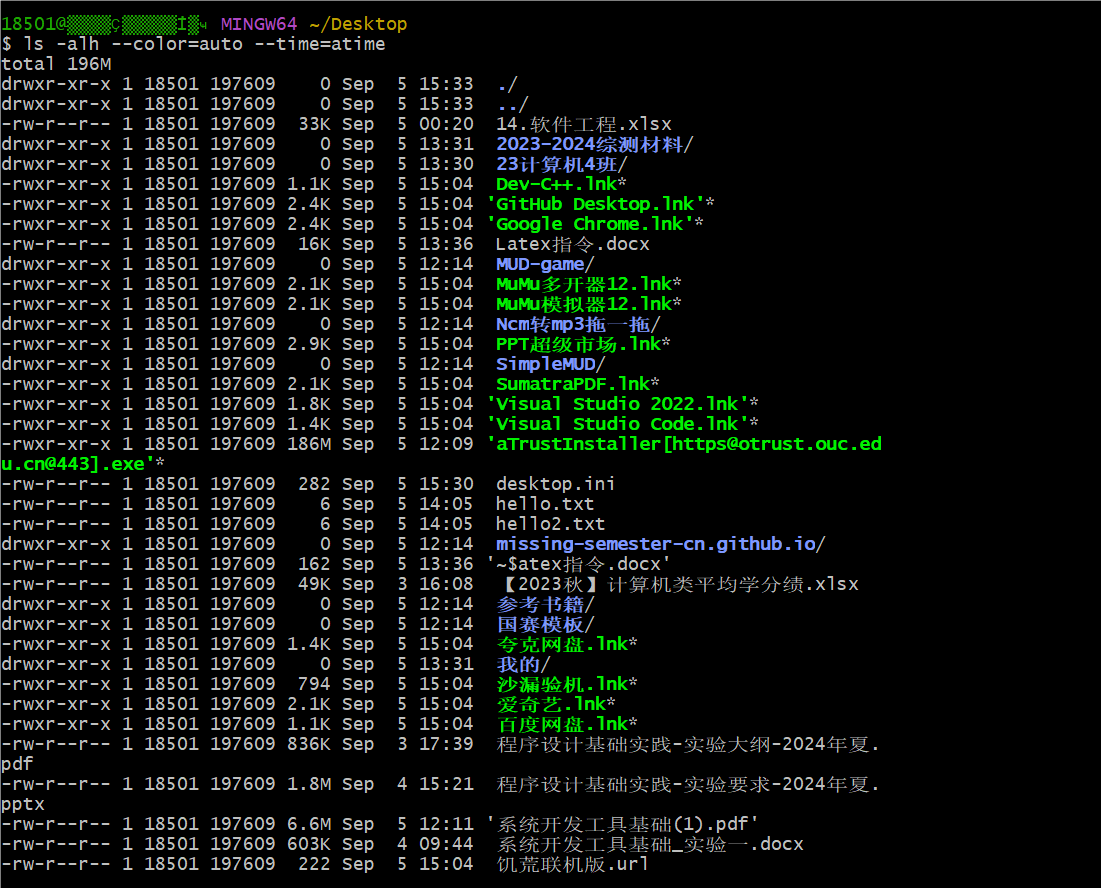
\includegraphics[width=14cm]{e96ab6acaa1341245480329c26f00d25.png}
        \caption{第一题}
        \label{fig:1}
    \end{figure}
 
    \item 编写两个 bash 函数 marco 和 polo 执行下面的操作。 
    每当你执行 marco 时,当前的工作目录应当以某种形式保存,
    当执行 polo 时,无论现在处在什么目录下,
    都应当 cd 回到当时执行 marco 的目录。 
    \begin{figure}[H]
        \centering
        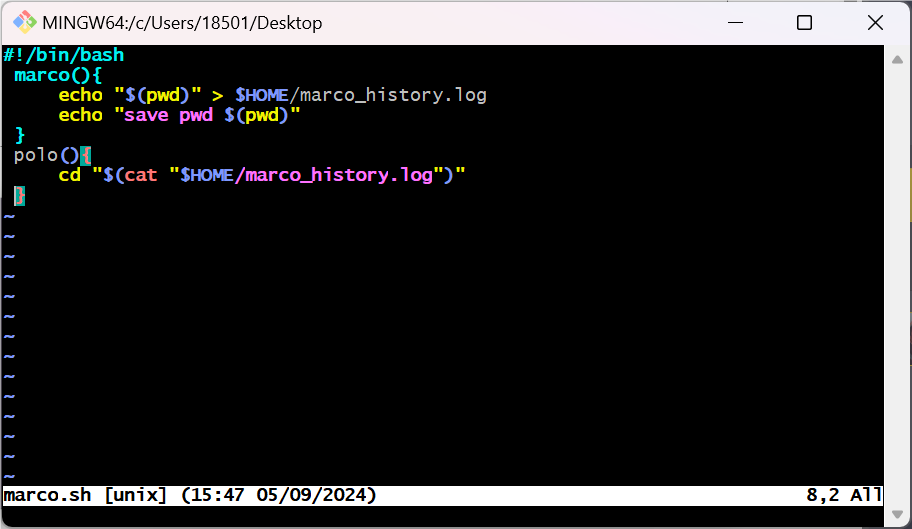
\includegraphics[width=14cm]{970751e5be9e298738cb2a7ab2044abe.png}
        \caption{编辑marco.sh文件中内容}
        \label{fig:1}
    \end{figure}
    \begin{figure}[H]
        \centering
        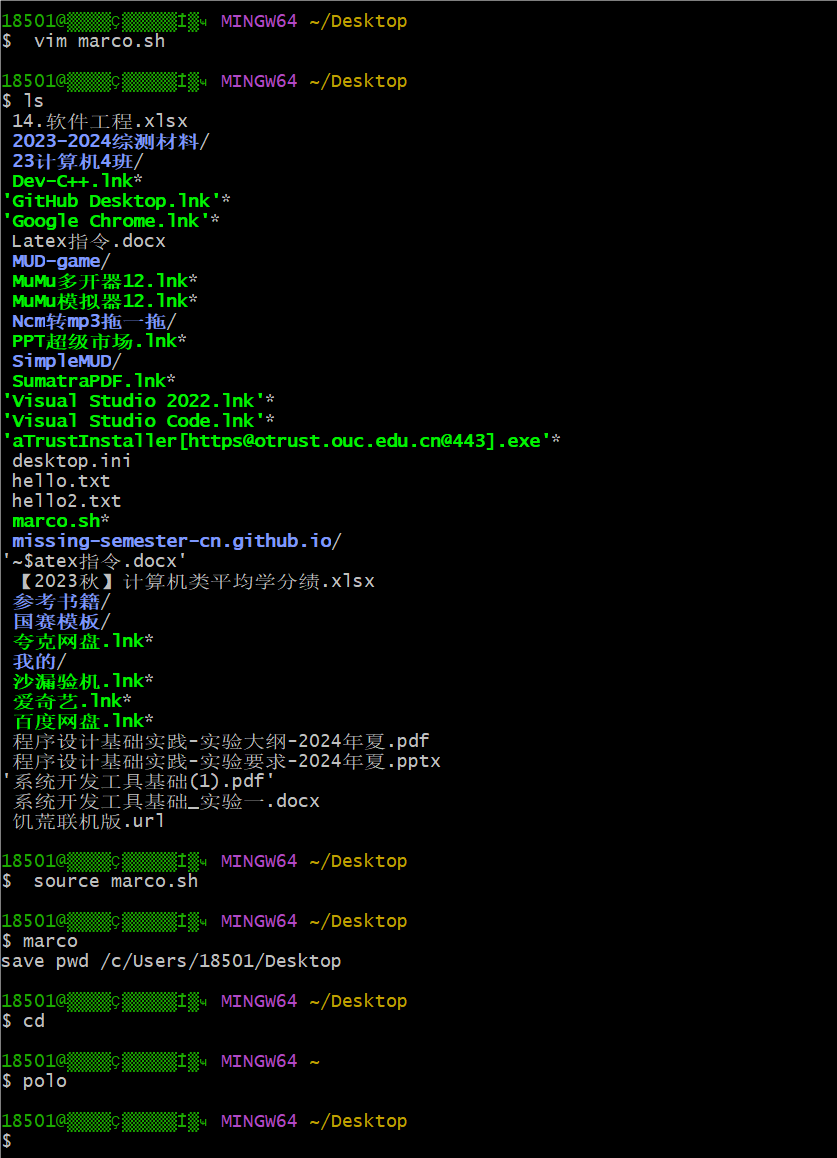
\includegraphics[width=14cm]{97009db96526e1ae888632d43c49af79.png}
        \caption{测试代码,成功运行}
        \label{fig:1}
    \end{figure}

    \item  编写一段bash脚本,运行脚本直到它出错,
    将它的标准输出和标准错误流记录到文件,并在最后输出所有内容。\\
    首先,创建一个test.sh文件编写以下脚本:\\
    \begin{figure}[H]
       \centering
       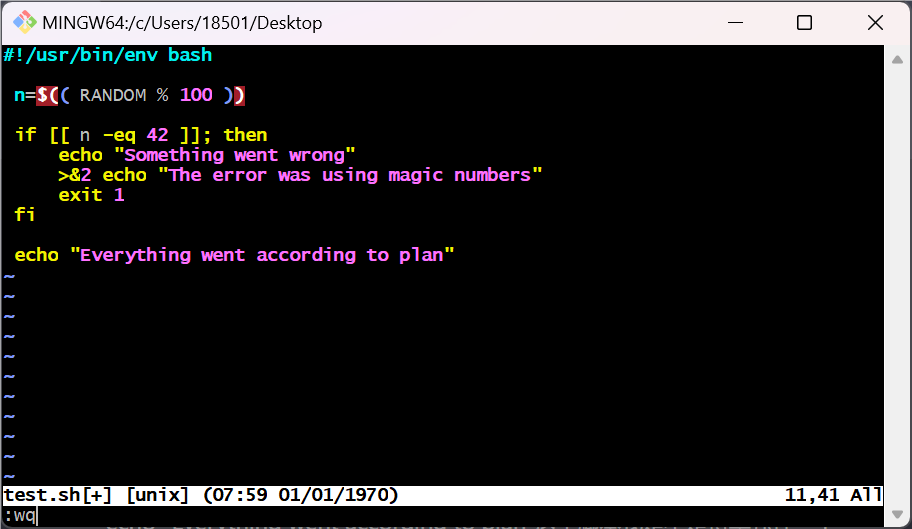
\includegraphics[width=14cm]{5fef4a7247b016a0fcaa02091262145c.png}
       \caption{编写test.sh脚本}
       \label{fig:3}
   \end{figure}
   然后,编写bash脚本,使用while循环完成:\\
   \begin{figure}[H]
    \centering
    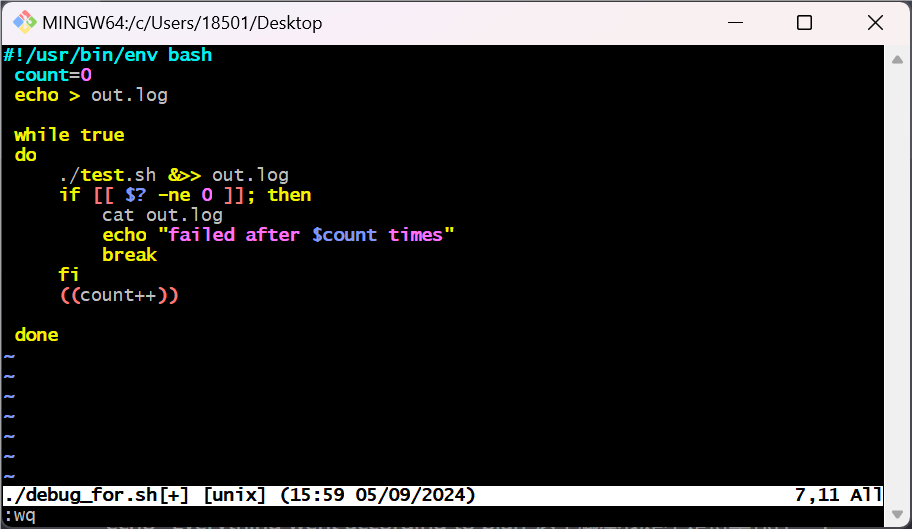
\includegraphics[width=14cm]{8948ac2ccd139bf852cab4120aa894c4.png}
    \caption{编写debug\_for.sh脚本}
    \label{fig:3}
    \end{figure}

    最后,执行测试脚本debug\_for.sh,并验证脚本结果的正确性:\\
\begin{figure}[H]
    \centering
    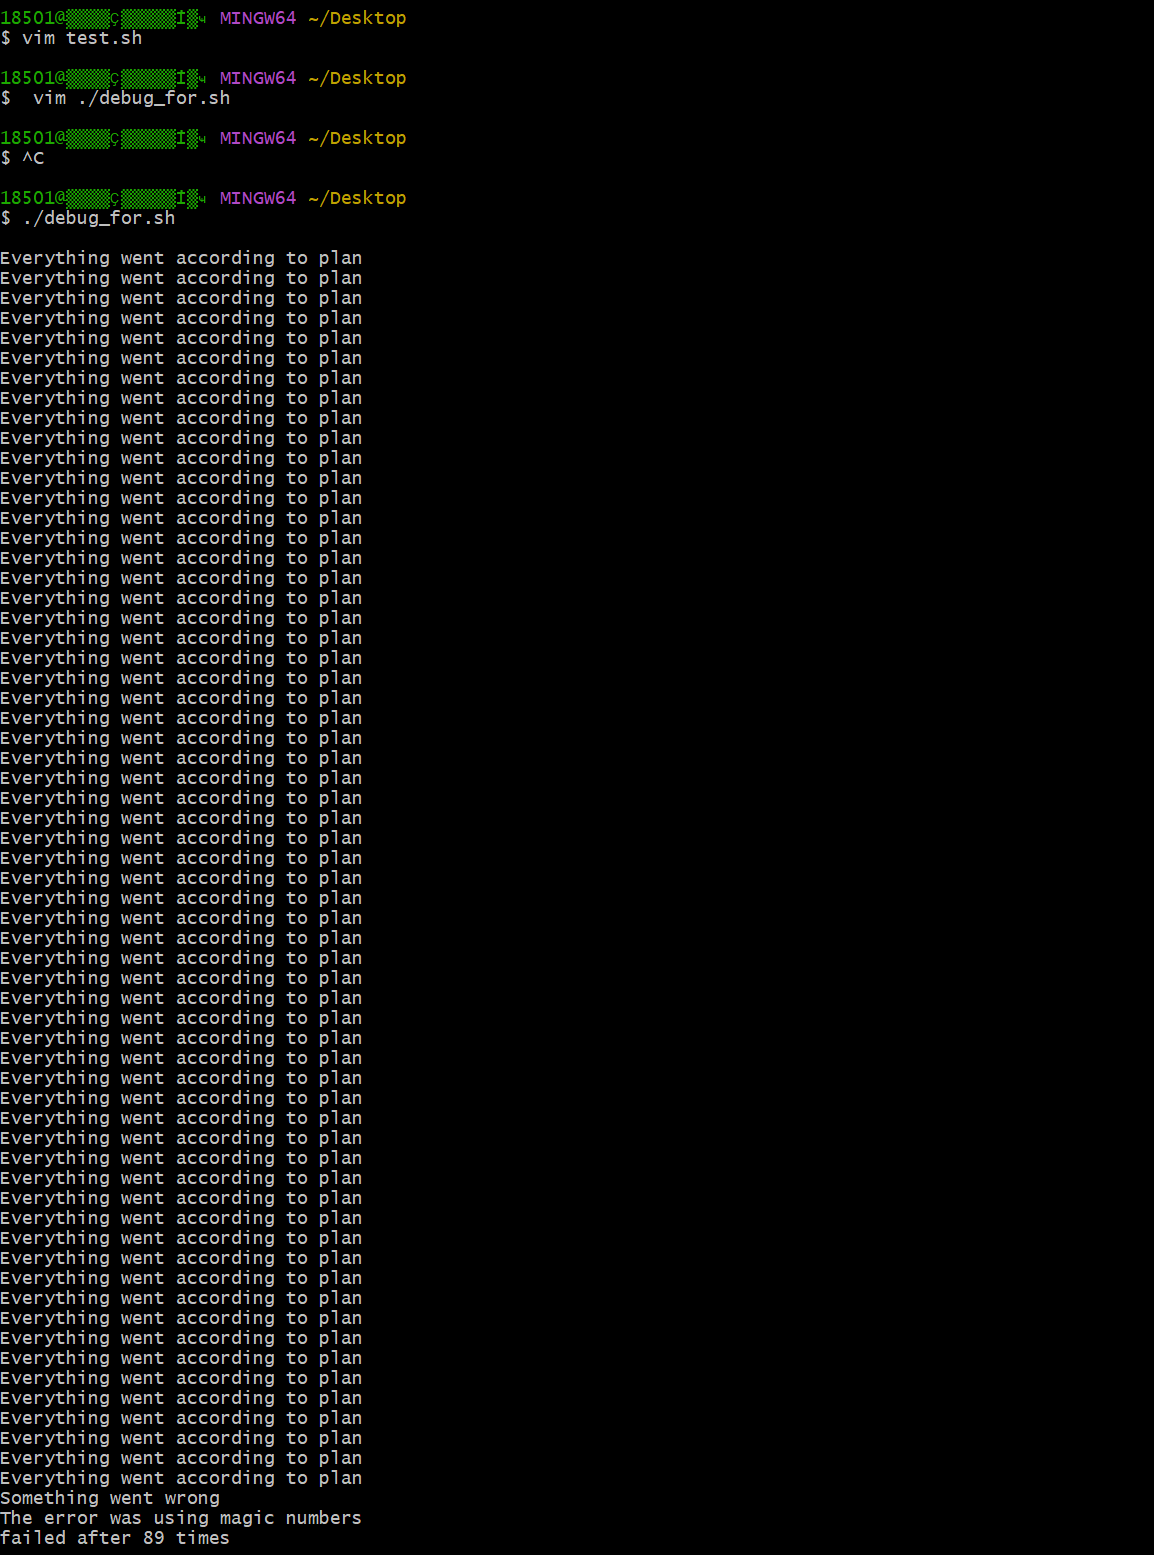
\includegraphics[width=14cm]{4c5ec2d33e22bdcedd1487fe534c4e52.png}
    \caption{执行脚本}
    \label{fig:3}
\end{figure}

\begin{figure}[H]
    \centering
    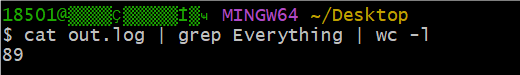
\includegraphics[width=14cm]{da5fa2fa70efc6918817e5af237e38dd.png}
    \caption{执行脚本}
    \label{fig:3}
\end{figure}

\end{enumerate}

\subsection{数据整理}
\begin{enumerate}
    \item  统计word文件中包含至少三个a 且不以's 结尾的单词个数\\
    大小写转换:
    \begin{lstlisting}
        tr "[:upper:]" "[:lower:]" 
        \end{lstlisting}
    查找一个以 a 结尾的字符串三次:
    \begin{lstlisting}
        ^([^a]a){3}.[^'s]$
        \end{lstlisting}
    匹配结尾为’s 的结果,然后取反:
        \begin{lstlisting}
            grep -v "'s$"
            \end{lstlisting}
    \begin{figure}[H]
       \centering
       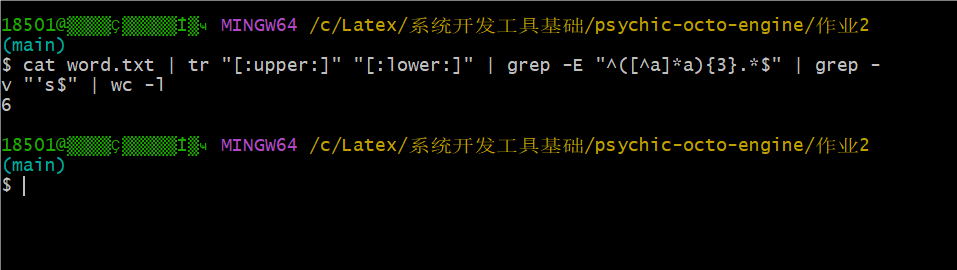
\includegraphics[width=14cm]{b5330fb548798ea1133829ff684385ea.png}
       \caption{至少三个a 且不以's 结尾的单词个数}
       \label{fig:3}
   \end{figure}
   \item  统计word文件中共存在多少种词尾两字母组合\\
   \begin{figure}[H]
    \centering
    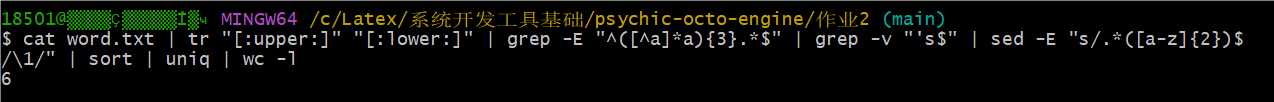
\includegraphics[width=14cm]{609a841f96213fe23a92fb328338af93.png}
    \caption{存在多少种词尾两字母组合}
    \label{fig:3}
\end{figure}
    \item  备份文件,自动创建一个后缀为 .bak 的备份文件\\
    \begin{figure}[H]
     \centering
     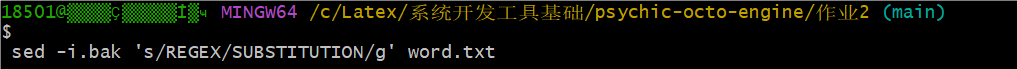
\includegraphics[width=14cm]{b342240e131500e7d40bf6cda43255e9.png}
     \caption{备份文件}
     \label{fig:3}

\end{figure}

\end{enumerate}
\section{练习实例}

\subsection{Shell工具和脚本}
\begin{enumerate}

    \item 初步使用Shell
    \begin{figure}[H]
       \centering
       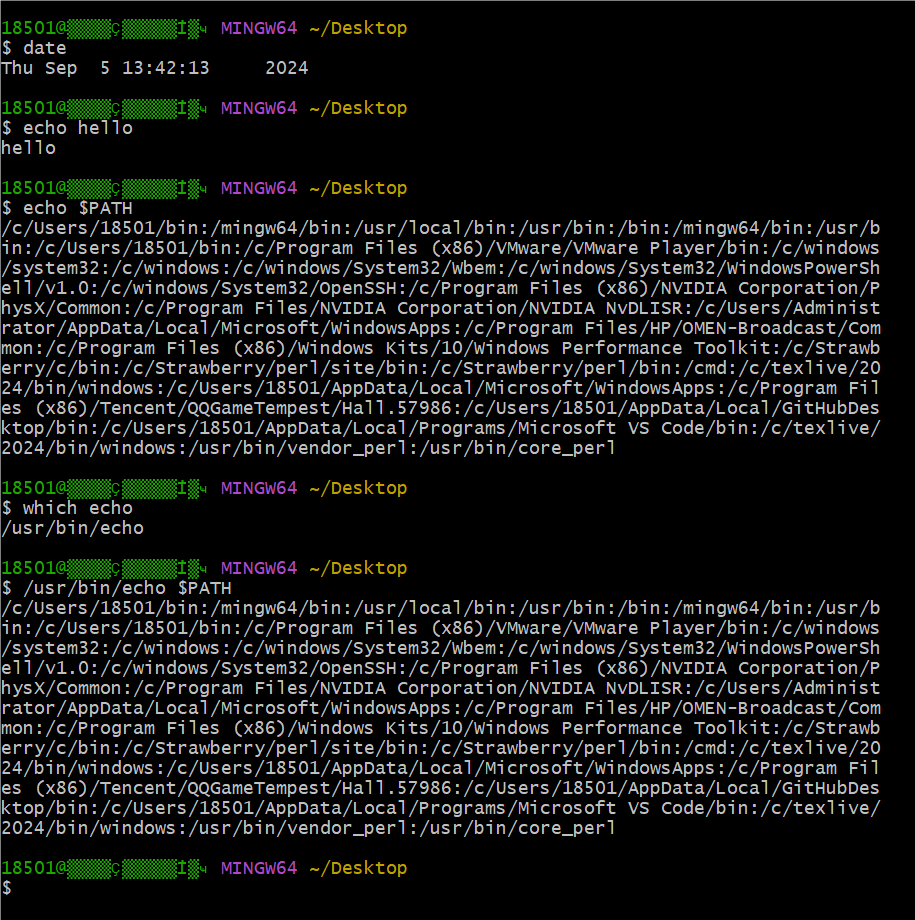
\includegraphics[width=10cm]{7a9723eb10f53b641242870e5b413206.png}
       \caption{初步使用Shell}
       \label{fig:1}
   \end{figure}

   \item pwd:获取当前工作目录
   \begin{figure}[H]
      \centering
      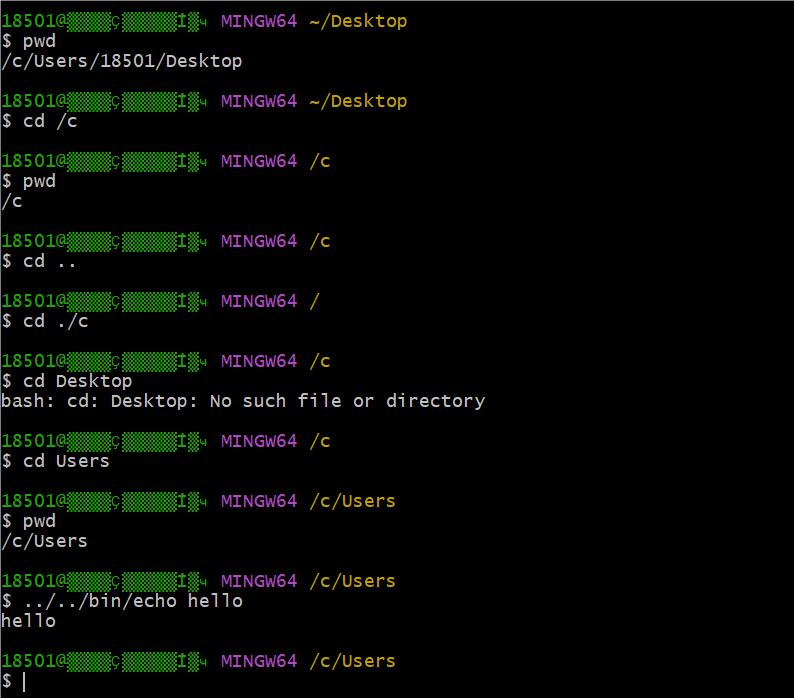
\includegraphics[width=10cm]{283139ae649fc8096bbc940266895d08.png}
      \caption{pwd学习与使用}
      \label{fig:2}
  \end{figure}

  \item 在程序间创建连接
  \begin{figure}[H]
     \centering
     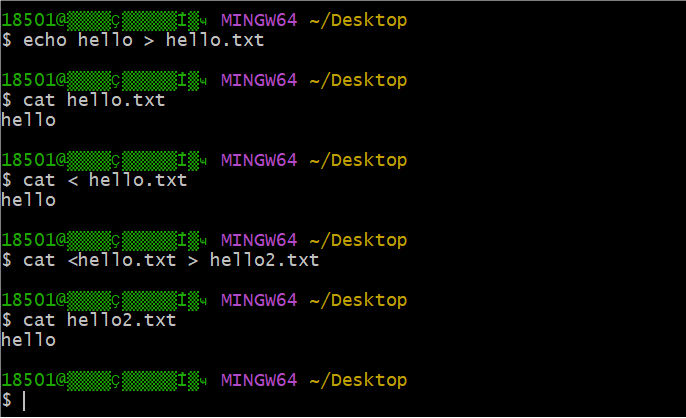
\includegraphics[width=10cm]{7d83e34fe5dbaf8dc4993da380f66ebf.png}
     \caption{}
     \label{fig:3}
 \end{figure}

 \item Shell写一个简单代码
 \begin{figure}[H]
    \centering
    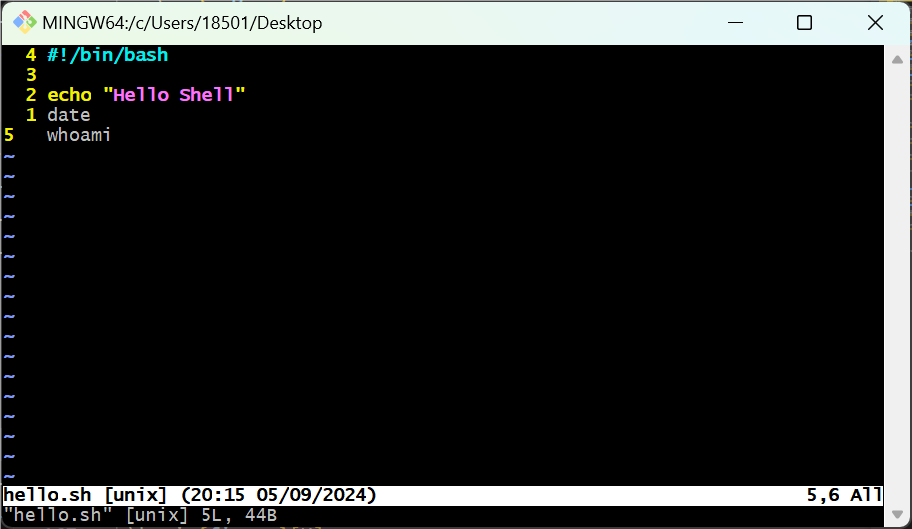
\includegraphics[width=10cm]{30de7a46c6cf548c2a7197eecba96203.png}
    \caption{编辑代码}
    \label{fig:3}
\end{figure}
 \begin{figure}[H]
    \centering
    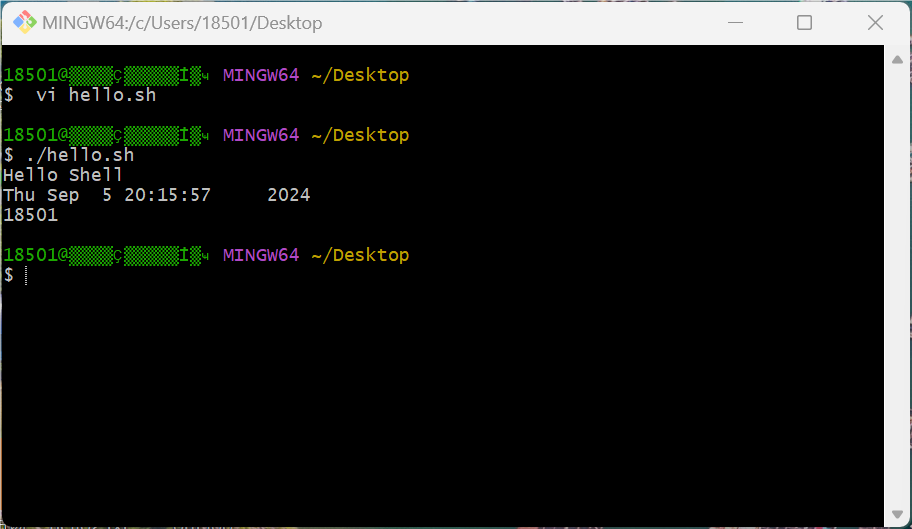
\includegraphics[width=10cm]{b1394dbef03c95aff4c1ac265715c22f.png}
    \caption{运行效果}
    \label{fig:3}
\end{figure}

\item Shell写一个猜数字游戏
 \begin{figure}[H]
    \centering
    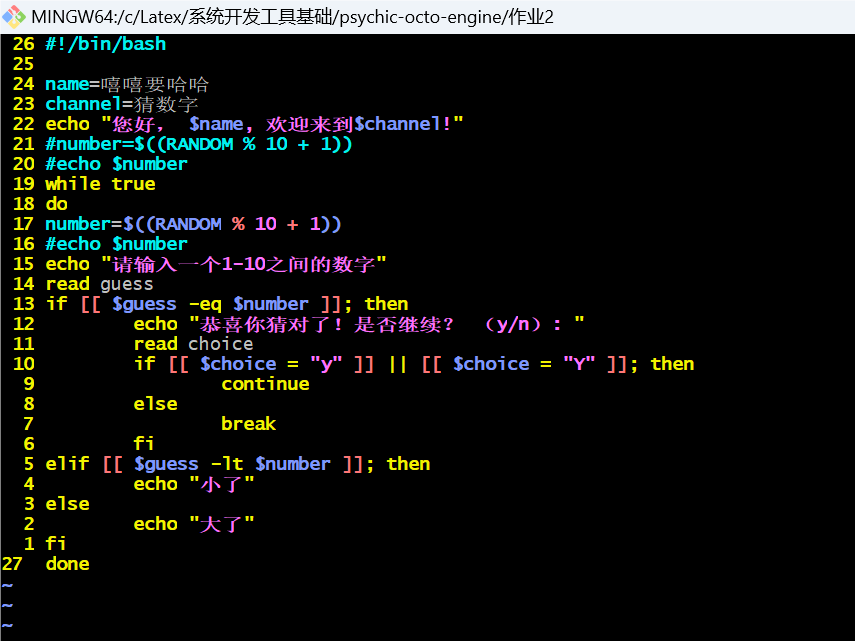
\includegraphics[width=12cm]{67c896cf1a6bfa021dca165852c2e7ca.png}
    \caption{编辑代码}
    \label{fig:3}
\end{figure}
\begin{figure}[H]
    \centering
    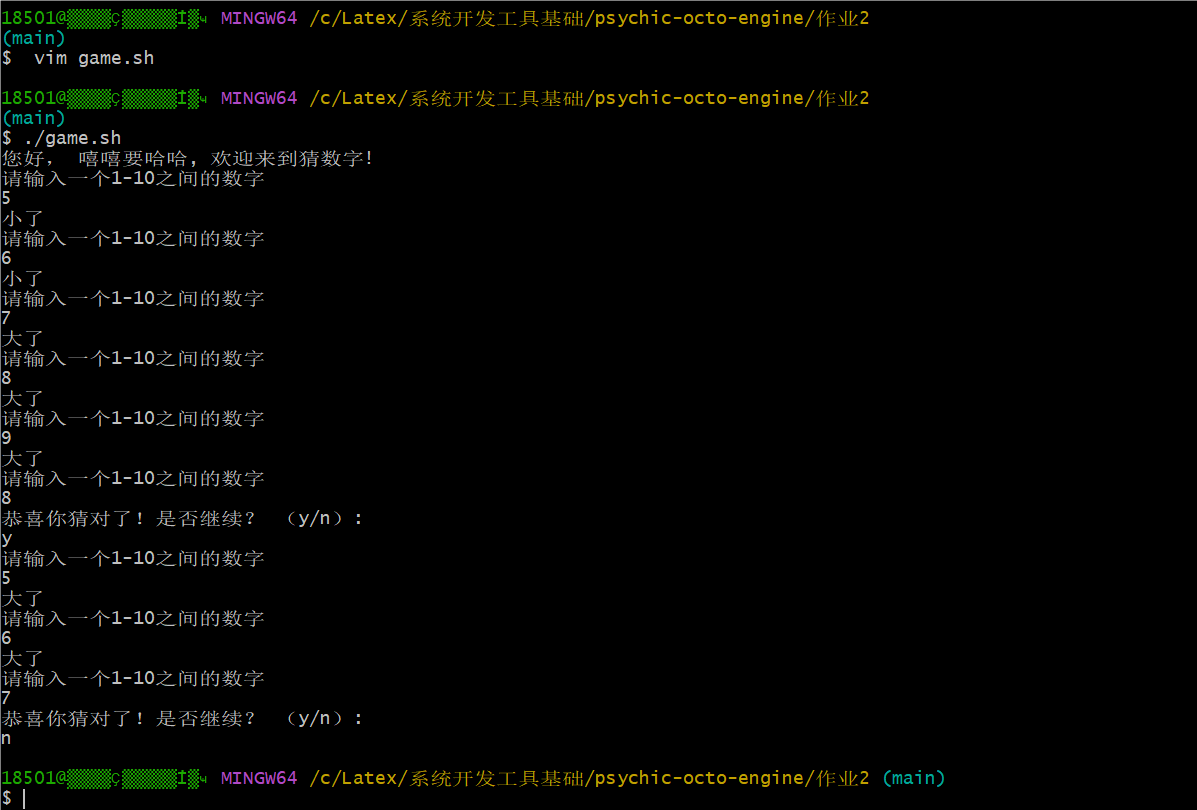
\includegraphics[width=12cm]{cfac9adf2cf508af7504105c35e1d837.png}
    \caption{运行效果}
    \label{fig:3}
\end{figure}
\end{enumerate}

\subsection{编辑器(Vim)}
\begin{enumerate}
    \item 显示编辑器行号与相对行号\\
    首先,检查vim版本\\
    \begin{figure}[H]
       \centering
       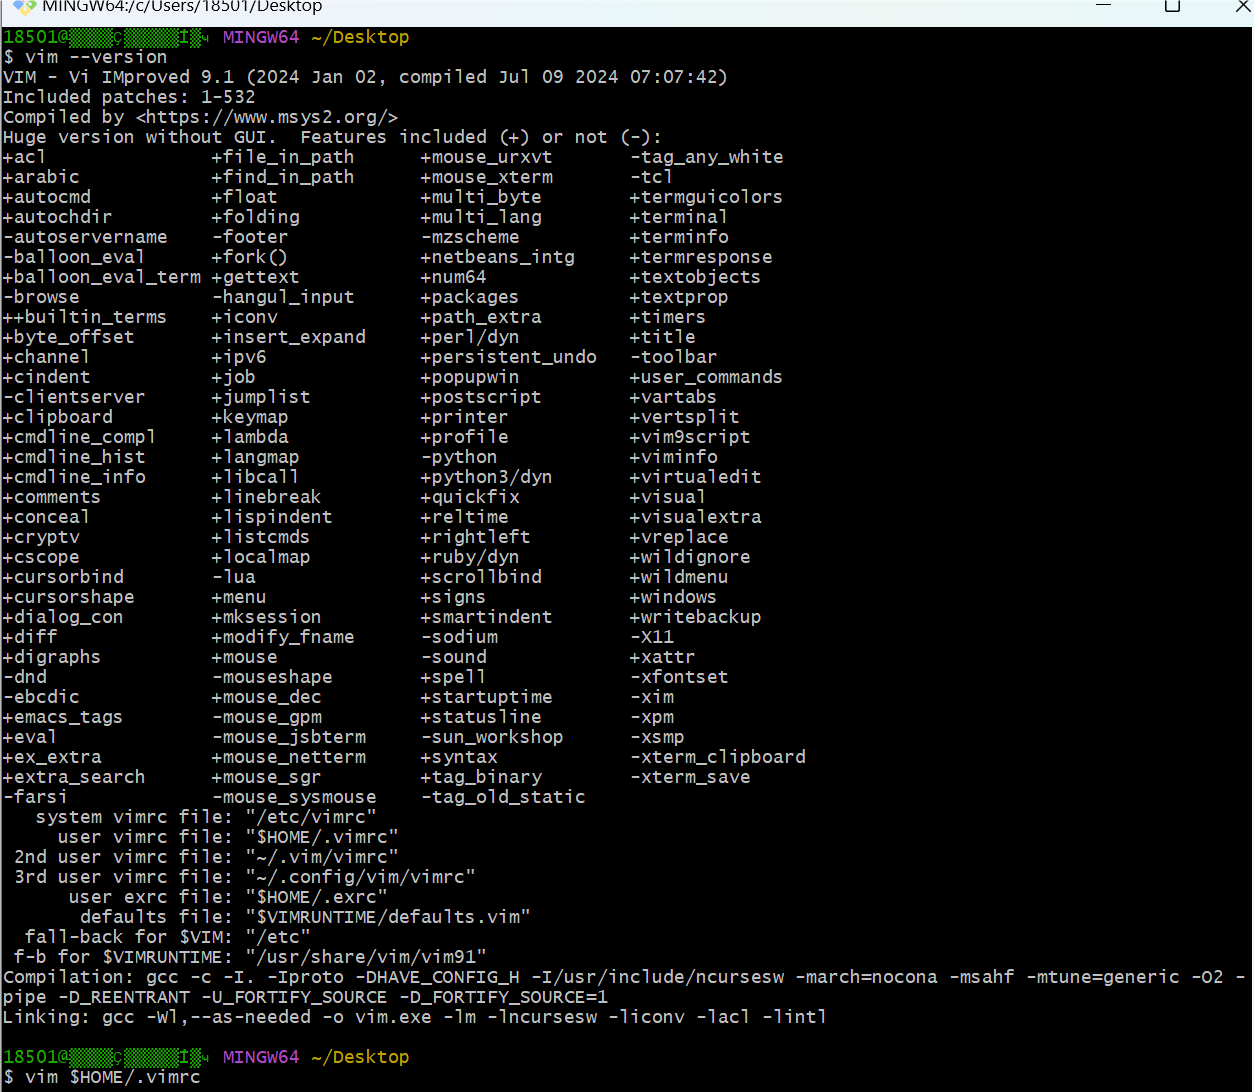
\includegraphics[width=14cm]{7ab83e3cf740c5a883a0b180edad18bf.png}
       \caption{检查vim版本}
       \label{fig:2}
   \end{figure}
   接着,找到并打开 \$HOME/.vimrc,添加如下代码:\\
   \begin{figure}[H]
    \centering
    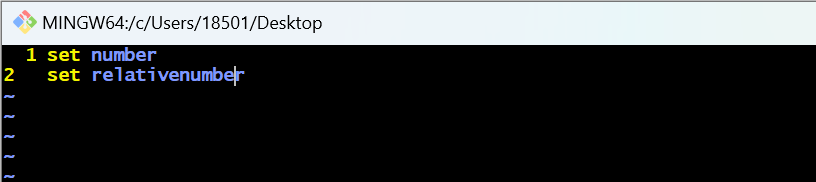
\includegraphics[width=14cm]{aab8e4332690e46b2e4f42720441a268.png}
    \caption{显示行号,相对行号的代码}
    \label{fig:2}
    \end{figure}
    效果如下:
    \begin{figure}[H]
        \centering
        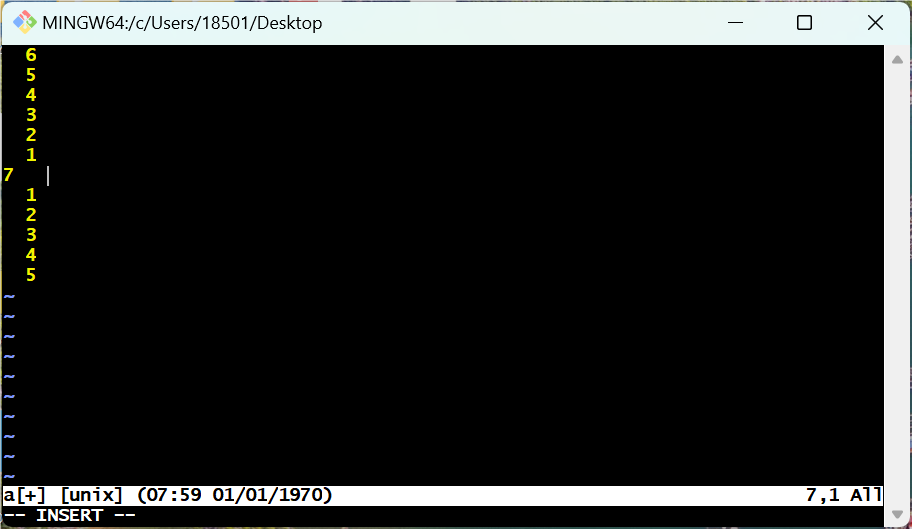
\includegraphics[width=14cm]{ac42008faf4a3fbf2da932e7ddb25f4d.png}
        \caption{效果如图}
        \label{fig:2}
    \end{figure}


\end{enumerate}
\subsection{数据整理}
一些由正则表达式的基本元素组合而成的例子
\begin{enumerate}
    \item 匹配电子邮件地址
    \begin{lstlisting}
        ^[a-zA-Z0-9._%+-]+@[a-zA-Z0-9.-]+\.[a-zA-Z]{2,}$
        \end{lstlisting}

    \item 匹配一个美国格式的电话号码(区号-三位数-四位数)
    \begin{lstlisting}
        ^[a-zA-Z0-9._%+-]+@[a-zA-Z0-9.-]+\.[a-zA-Z]{2,}$
        \end{lstlisting}

    \item 匹配电子邮件地址
    \begin{lstlisting}
        ^\d{3}-\d{3}-\d{4}$
        \end{lstlisting}

    \item 匹配URL
    \begin{lstlisting}
        ^(http|https)://[a-zA-Z0-9.-]+(:\d+)?(/[a-zA-Z0-9._?%&=-]*)?$
        \end{lstlisting}

        \item 匹配中文字符
    \begin{lstlisting}
        ^[\u4e00-\u9fa5]+$
        \end{lstlisting}

        \item 匹配一个 YYYY-MM-DD 格式的日期
    \begin{lstlisting}
        ^\d{4}-\d{2}-\d{2}$
        \end{lstlisting}
\end{enumerate}
\section{实验心得}
学习 Shell 语法、Vim 编辑器的使用以及正则表达式的掌握对于我们这种
从事编程、系统管理或日常脚本开发的人来说是非常重要的技能,对于我们在未来无论是
科研竞赛抑或是工作上都是有不小的帮助的。这学习的过程中我也体会颇多。
\subsection{Shell}
\begin{itemize}
\item 自动化能力:掌握了 Shell 脚本的基础之后,我们便可以编写简单的自动化任务,如文件备份、定时任务、数据处理等。\\
\item 环境控制:Shell 脚本可以让我们更好地控制系统环境,包括启动服务、停止进程、监控资源使用等。\\
\item 命令行效率:熟悉 Shell 命令和管道 (|)、重定向 (>, >>) 等概念,可以提高我们在命令行界面工作的效率。\\
\end{itemize}
很重要的一点是,shell对于格式的要求很严格,对于空格等有非常明确的判定规则,对于我们初学者时常会在这个方面犯错而久久找不到问题所在。\\
\subsection{Vim 编辑器}
\begin{itemize}
    \item 高效编辑:Vim 的模式切换(普通模式、插入模式、命令行模式)使得文本编辑更加高效,尤其是通过键盘快捷键进行光标移动、文本选择、删除和复制等操作。\\
    \item 跨平台性:Vim 几乎在所有操作系统上都可以使用,这对于需要在不同平台上进行开发的人来说非常有用。\\
    \end{itemize}
    我以后在日常使用中尽量使用 Vim,逐渐习惯其操作方式。
\subsection{数据整理}
\begin{itemize}
    \item 精确匹配:正则表达式可以让你非常精确地匹配和处理文本中的模式,无论是查找、替换还是提取信息都非常方便。\\
    \item 灵活性:正则表达式的灵活性非常高,几乎可以用来匹配任何文本模式。\\
    \end{itemize}

\section{Github仓库ssh链接}
 \url {git@github.com:xixiyhaha/psychic-octo-engine.git }
\end{document}